\documentclass{tufte-handout}
\usepackage[utf8]{inputenc}
\usepackage[francais]{babel}

\title{Manuel d'utilisation du simulateur ARM epater\\Révision 1}


\author{Marc-André Gardner\\Yannick Hold-Geoffroy\\Jean-François Lalonde}

%\date{28 March 2010} % without \date command, current date is supplied

%\geometry{showframe} % display margins for debugging page layout

\usepackage{graphicx} % allow embedded images
  \setkeys{Gin}{width=\linewidth,totalheight=\textheight,keepaspectratio}
  \graphicspath{{graphics/}} % set of paths to search for images
\usepackage{amsmath}  % extended mathematics
\usepackage{booktabs} % book-quality tables
\usepackage{units}    % non-stacked fractions and better unit spacing
\usepackage{multicol} % multiple column layout facilities
\usepackage{lipsum}   % filler text
\usepackage{fancyvrb} % extended verbatim environments
  \fvset{fontsize=\normalsize}% default font size for fancy-verbatim environments

% Standardize command font styles and environments
\newcommand{\doccmd}[1]{\texttt{\textbackslash#1}}% command name -- adds backslash automatically
\newcommand{\docopt}[1]{\ensuremath{\langle}\textrm{\textit{#1}}\ensuremath{\rangle}}% optional command argument
\newcommand{\docarg}[1]{\textrm{\textit{#1}}}% (required) command argument
\newcommand{\docenv}[1]{\textsf{#1}}% environment name
\newcommand{\docpkg}[1]{\texttt{#1}}% package name
\newcommand{\doccls}[1]{\texttt{#1}}% document class name
\newcommand{\docclsopt}[1]{\texttt{#1}}% document class option name
\newenvironment{docspec}{\begin{quote}\noindent}{\end{quote}}% command specification environment
\usepackage{hyperref}


\usepackage{color}


\begin{document}

\maketitle% this prints the handout title, author, and date


\section{Introduction}

Ce manuel présente l'utilisation du simulateur \textbf{épater}, qui émule un processeur à architecture ARMv7, tel qu'étudié dans le cours \textit{GIF-1001 Ordinateurs: Structure et Applications}. Ce manuel se concentre uniquement sur l'utilisation du simulateur à proprement parler. Les informations concernant l'architecture ARM et la programmation en langage assembleur peuvent être obtenues dans les notes de cours ou dans les manuels de référence cités dans le plan de cours.

\section{Prise en main}

\subsection{Accès au simulateur}

Le simulateur est disponible en ligne, à l'adresse \url{http://gif1001-sim.gel.ulaval.ca/}. Aucune installation n'est nécessaire et l'accès ne requiert pas d'authentification. Le simulateur a été testé avec les navigateurs suivants :
\begin{itemize}
	\item Google Chrome version 50 et plus, sur Windows, MacOS et Linux
	\item Mozilla Firefox version 44 et plus, sur Windows, MacOS et Linux
	\item Microsoft Edge, sur Windows 10
	\item Apple Safari, sur MacOS
\end{itemize}

D'autres navigateurs peuvent également être compatibles avec l'interface du simulateur, mais cette compatibilité n'est pas garantie. Si vous rencontrez des problèmes avec un navigateur alternatif, installez un des navigateurs énumérés plus haut.

\subsection{Enregistrement et chargement}

\paragraph{\textbf{\color{red}{Note importante :}}} \textbf{\color{red}{Le serveur ne réalise \emph{aucune} sauvegarde de votre code ou de vos données. Il est de \emph{votre} responsabilité de télécharger le fichier contenant votre code à chaque fois que vous quittez la session de simulation ou fermez votre navigateur.}}

\section{Utilisation du simulateur}

La page d'accueil du simulateur est présentée à la figure \ref{f:accueil}. Elle contient, sur la gauche, un menu permettant de choisir le type d'activité (démonstrations, exercices, travaux pratiques ou codage libre) et, dans sa section principale, une liste des programmes disponibles.

\begin{figure}
\raggedleft
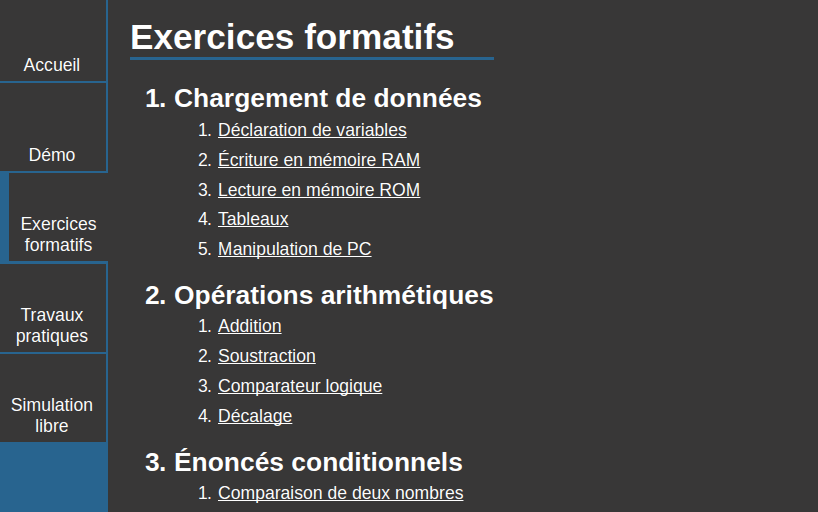
\includegraphics[width=0.7\linewidth]{pics/accueil.png}
\label{f:accueil}
\caption{Page d'accueil du simulateur}
\end{figure}

Cliquer sur l'un de ces programmes ouvre l'interface de simulation à proprement parler. La figure \ref{f:global} présente un exemple typique de cette interface, annotée. Les sous-sections suivantes présentent chaque zone de l'interface.

\begin{figure*}[h!]
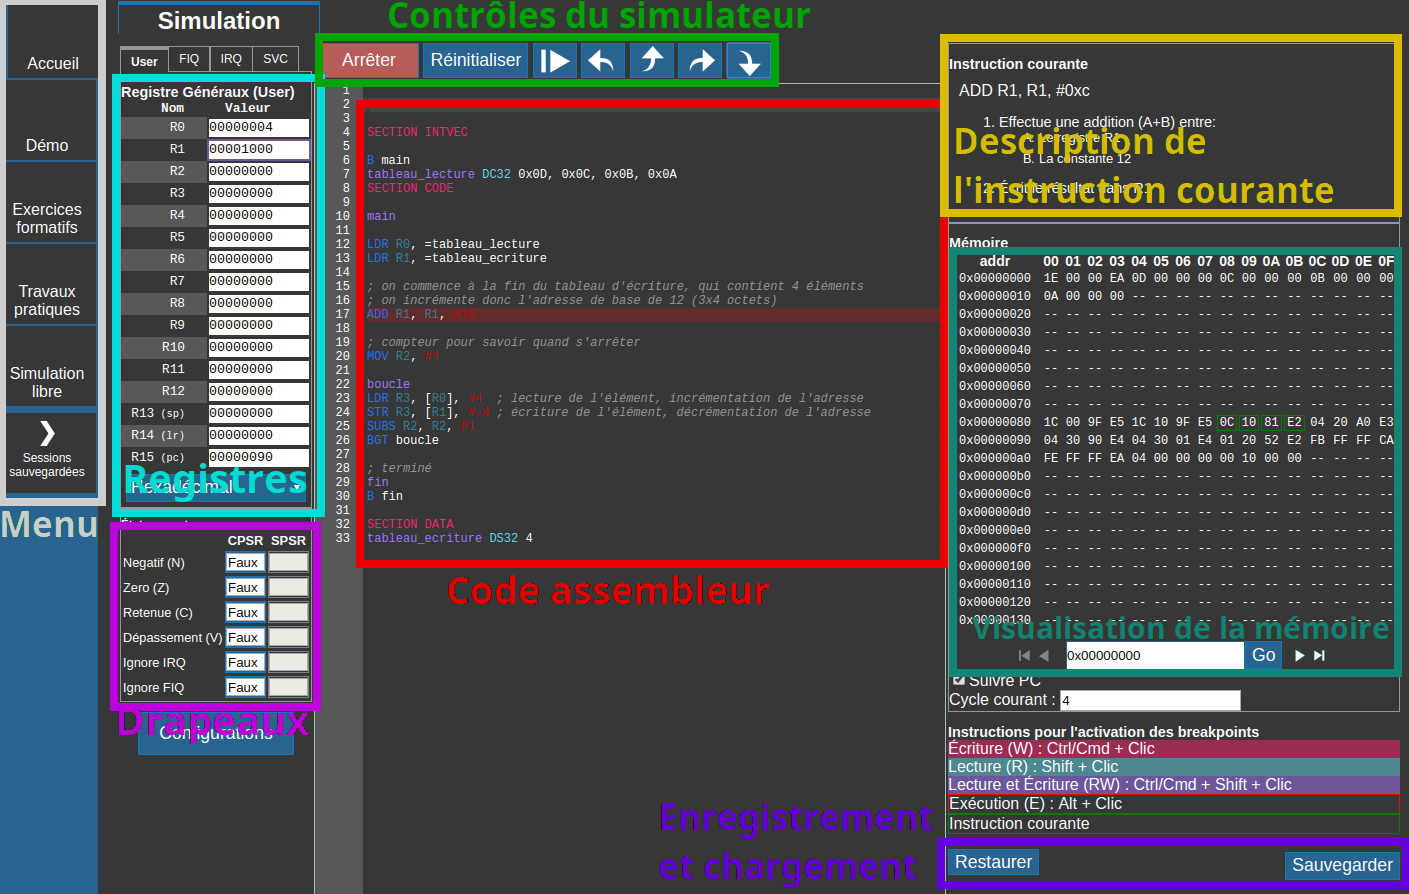
\includegraphics[width=0.86\linewidth]{pics/main_labeled.png}
\label{f:global}
\caption{Vue d'ensemble de l'interface du simulateur.}
\end{figure*}

\clearpage

\subsection{Éditeur de code}

\begin{marginfigure}
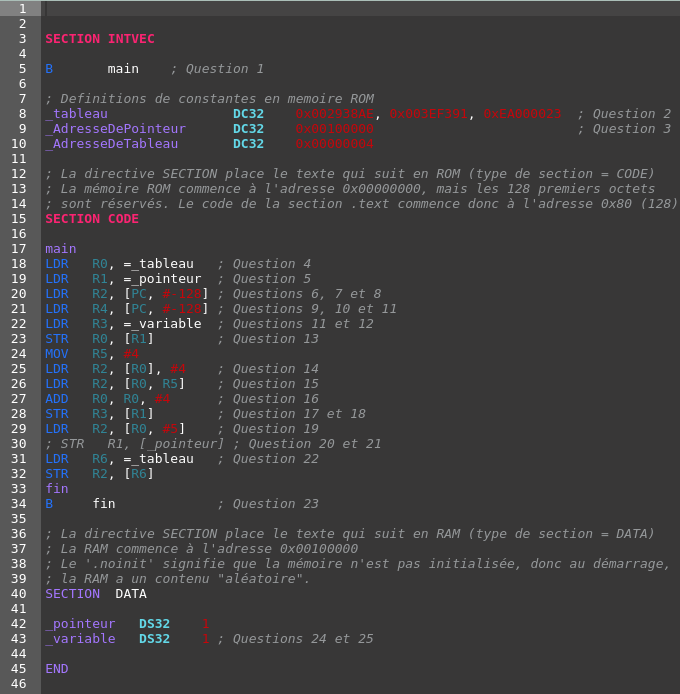
\includegraphics[width=\linewidth]{pics/editeur.png}
\label{f:editeur}
\caption{Vue typique de l'éditeur}
\end{marginfigure}
L'éditeur de code constitue la zone principale du simulateur. C'est dans cet éditeur que vous pouvez créer votre programme. Lors de l'exécution, \emph{l'éditeur passe en mode lecture seulement}, mais présente certaines informations comme la ligne en cours d'exécution.

Cet éditeur possède une \emph{coloration syntaxique}, c'est-à-dire qu'il est capable d'analyser le code qu'il convient pour colorier différemment les diverses parties d'une instructions. Cela permet de faciliter la lecture et la détection des erreurs. 

La colonne de gauche contient le numéro de ligne. Lorsqu'une instruction est erronée, un X blanc sur fond rouge y apparaît pour signaler le problème :
\begin{figure}[h!]
\raggedleft
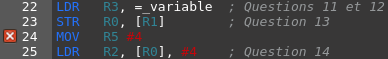
\includegraphics[width=0.9\linewidth]{pics/editeur_err.png}
\label{f:editeurerror}
\caption{Exemple d'instruction erronée. Le X blanc sur fond rouge signale la ligne contenant l'instruction invalide.}
\end{figure}

Passer la souris sur ce X fait apparaître une infobulle contenant un texte explicatif de l'erreur :
\begin{figure}[h!]
\raggedleft
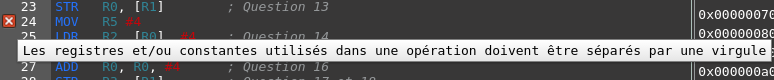
\includegraphics[width=\linewidth]{pics/editeur_err_bulle.png}
\label{f:editeurerrorplus}
\caption{Le message expliquant l'erreur peut être consulté en passant la souris sur le X.}
\end{figure}

Une fois le programme \emph{assemblé} (le bouton ``Démarré'' pressé et le code assemblé sans erreur), il est possible de mettre en place des points d'arrêt (\textit{breakpoints}) en cliquant sur le numéro d'une ligne. Un point d'arrêt force le simulateur à s'arrêter lorsqu'il l'atteint. Un point d'arrêt peut être désactivé en recliquant sur le même numéro de ligne. Par exemple, dans la figure suivante, les lignes 20 et 22 sont des points d'arrêt :
\begin{figure}[h!]
\raggedleft
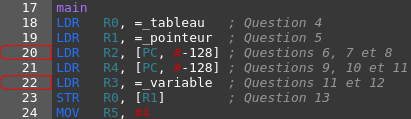
\includegraphics[width=0.9\linewidth]{pics/editeur_bkpt.png}
\label{f:editeurbkpt}
\caption{Un point d'arrêt (\textit{breakpoint}) peut être mis en place en cliquant sur le numéro de ligne, une fois le programme assemblé.}
\end{figure}

\paragraph{\textbf{Note importante :}}un point d'arrêt ne peut être placé que sur une ligne \emph{contenant une instruction}. Si l'utilisateur clique sur une ligne ne contenant pas d'instructions, le point d'arrêt sera placé sur la prochaine ligne contenant une instruction. Par exemple, à la figure \ref{f:editeurbkpt}, cliquer sur la ligne 17 placera un point d'arrêt à la ligne \emph{18}.

Lors de l'exécution, l'éditeur passe en mode lecture seule. Il affiche cependant certaines informations. La ligne en cours d'exécution est surlignée en rouge bourgogne :
\begin{figure}[h!]
\raggedleft
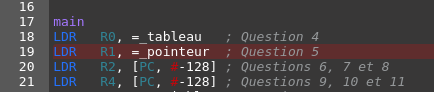
\includegraphics[width=0.9\linewidth]{pics/editeur_lignecourante.png}
\label{f:editeurlignecourante}
\caption{L'instruction qui va être exécutée au prochain pas de temps est surlignée en rouge dans l'éditeur. Si aucune instruction n'est surlignée, c'est que le \textit{Program Counter} (PC) ne se situe pas dans la mémoire d'instructions.}
\end{figure}

De même, lorsque l'instruction courante est un branchement ou un appel de fonction, l'éditeur affiche la destination du branchement en surlignant en noir la prochaine instruction. Par exemple, dans ce cas-ci, l'instruction en cours d'exécution (surlignée en rouge) est le \textit{B main}, et la prochaine instruction sera celle de la ligne 18 (surlignée en noir) :
\begin{figure}[h!]
\raggedleft
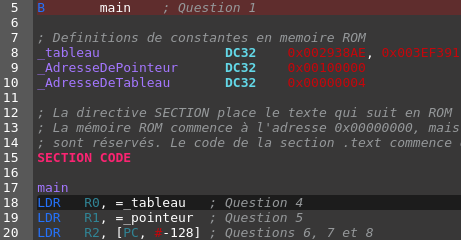
\includegraphics[width=0.9\linewidth]{pics/editeur_prediction.png}
\label{f:editeurbranch}
\caption{La prochaine instruction à être exécutée après un branchement est surlignée en noir profond. Si le branchement est conditionnel, cet affichage en tient compte et affiche la prochaine instruction correspondant à la branche prise.}
\end{figure}

\clearpage

\subsection{Contrôles du simulateur}

Les boutons de contrôle du simulateur permettent d'agir sur la simulation. 
Cette interface diffère selon le mode actuel. Dans le mode \emph{édition} (figure~\ref{f:controles1}), seul le bouton \textit{Démarrer} est actif. Dans le mode \emph{exécution}, que l'on peut accéder en pressant sur \textit{Démarrer}, tous les boutons sont actifs, et le bouton \textit{Démarrer} devient \textit{Arrêter}. 
\begin{figure}[h!]
\raggedleft

\includegraphics[width=0.8\linewidth]{pics/controles_1b.png}
\label{f:controles1}
\caption{Barre de contrôle en mode \emph{édition}}
\end{figure}
\begin{figure}[h!]
\raggedleft

\includegraphics[width=0.8\linewidth]{pics/controles_2b.png}
\label{f:controles2}
\caption{Barre de contrôle en mode \emph{exécution}}
\end{figure}

Lorsque le bouton \textit{Démarrer} est pressé, le simulateur tente d'abord d'assembler le code. Si aucune erreur n'est détectée, il passe alors en mode exécution. Dans ce mode, tous les boutons sont actifs et sont, respectivement, de gauche à droite :
\begin{enumerate}
	\item \textbf{Arrêt} : interrompt la simulation et revient en mode édition.
	\item \textbf{Réinitialisation} : effectue l'équivalent d'une interruption \emph{reset} sur le microprocesseur. La valeur de PC est mise à $0$. Notez que cela n'affecte \emph{pas} la valeur des autres registres et des drapeaux.
	\item \textbf{Exécution en continu} : le simulateur exécute les instructions suivantes sans arrêt, jusqu'à ce qu'il rencontre une erreur ou un point d'arrêt. Notez que le simulateur est volontairement limité quant au nombre d'instructions qu'il peut exécuter d'un seul coup. Lorsque ce nombre est atteint, le simulateur arrête comme s'il avait rencontré un point d'arrêt. Il suffit d'appuyer à nouveau sur le bouton d'exécution en continu pour poursuivre.
	\item \textbf{Exécuter instruction courante} : exécute l'instruction courante (celle qui est surlignée dans l'éditeur) et passe à la suivante puis arrête.
	\item \textbf{Exécuter ligne courante} : dans le cas où la ligne courante est une instruction autre que BL, cette action a le même effet que la précédente. Toutefois, dans le cas d'un appel de fonction (BL), cette action exécute l'entièreté de la fonction jusqu'à son retour.
	\item \textbf{Exécuter jusqu'à la sortie} : dans le cas où la ligne courante est dans une fonction, cette action exécute sans arrêt les instructions jusqu'à sortir de la fonction (appel de BX). Si la ligne courante n'est pas dans une fonction, cette action a le même effet qu'une exécution en continu.
\end{enumerate}

\clearpage

\subsection{Vue des registres}

\begin{marginfigure}
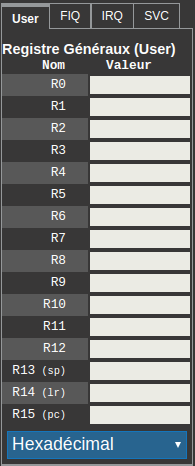
\includegraphics[width=0.8\linewidth]{pics/registres.png}
\label{f:registres}
\caption{Vue des registres généraux}
\end{marginfigure}
La section de gauche de l'interface présente les valeurs contenues dans les registres du processeur.
Les 16 registres que contient un processeur ARM (R0 à R15) sont affichés. 

Par défaut, leur valeur est présentée en hexadécimal, mais il est possible de choisir différents modes d'affichage en cliquant sur le mode actuel pour faire apparaître le menu de sélection. Le mode décimal signé correspond à une interprétation complément-2 de la valeur du registre, alors que le mode non-signé correspond à une simple conversion vers le système décimal.
\begin{marginfigure}
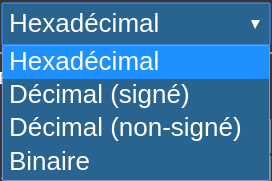
\includegraphics[width=0.8\linewidth]{pics/registres_format.png}
\label{f:regformat}
\caption{Menu de sélection du mode d'affichage}
\end{marginfigure}

Les onglets au-dessus des registres permettent de choisir la \textit{banque} de registre à visualiser. La plupart des banques de registre d'un processeur ARM sont présentes, incluant la banque IRQ (interruption), FIQ (interruption rapide) et SVC (interruption logicielle).
\begin{marginfigure}

\includegraphics[width=\linewidth]{pics/registres_banques.png}
\label{f:regbank}
\caption{Onglets de sélection de la banque de registres à visualiser}
\end{marginfigure}

La valeur d'un registre peut être modifiée en changeant sa valeur dans l'interface. Attention toutefois à respecter le type d'affichage sélectionné (par exemple, il est illégal d'écrire autre chose que 0 ou 1 en mode binaire).

Il est possible d'affecter un point d'arrêt à un registre, en mode lecture ou écriture. Un point d'arrêt lié à un registre met la simulation en pause lorsque le registre est écrit ou lu. Par exemple, dans la figure suivante, les registres R3 et R5 ont un point d'arrêt en écriture et le registre R2 un point d'arrêt en lecture :
\begin{marginfigure}
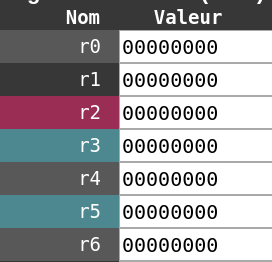
\includegraphics[width=0.8\linewidth]{pics/registres_bkpt.png}
\label{f:regbkpt}
\caption{Points d'arrêt sur les registres R2, R3 et R5.}
\end{marginfigure}

Un point d'arrêt en écriture peut être ajouté en cliquant sur le nom du registre tout en tenant la touche Ctrl ou Cmd enfoncée, respectivement sur Windows et MacOS. De même, un point d'arrêt en lecture peut être ajouté en cliquant tout en tenant la touche Maj (Shift) enfoncée. Un point d'arrêt précédemment créé peut être retiré en répétant la même opération. Il est possible de mettre à la fois un point d'arrêt en lecture et en écriture sur le même registre.

Lorsque l'instruction courante lit ou écrit un registre, sa valeur est entourée d'un rectangle turquoise (lecture) ou rouge (écriture). Par exemple, dans l'image suivante, l'instruction courante lit les valeurs de R0 et R5 et écrit dans R2 :
\begin{figure}[h!]
\raggedright
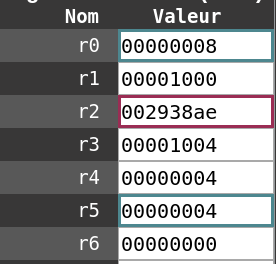
\includegraphics[width=0.38\linewidth]{pics/registres_statuts.png}
\label{f:regstatut}
\end{figure}

\clearpage

\subsection{Vue des drapeaux}

Les drapeaux de l'ALU sont présentés juste en dessous de la vue des registres.
\begin{marginfigure}
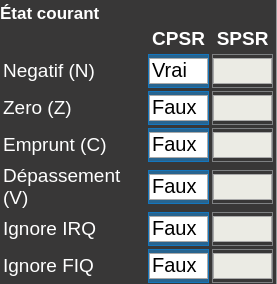
\includegraphics[width=0.9\linewidth]{pics/drapeaux.png}
\label{f:drapeaux}
\caption{Vue des drapeaux de l'ALU}
\end{marginfigure} 
Un drapeau ne peut prendre que deux valeurs : vrai ou faux (0 ou 1 en binaire). Il est possible de changer la valeur d'un drapeau en cliquant sur sa valeur. L'interface présente à la fois la vue pour le registre de statut courant (CPSR) et le registre de statut sauvegardé (SPSR), si applicable.

Le registre de statut sauvegardé (SPSR) est propre à chaque banque de registres, hormis la banque \textit{User} qui n'en possède pas. Il permet de conserver le registre de statut du programme principal pendant une interruption. Dans la majorité des cas (exécution en mode \textit{User}), les valeurs du SPSR ne sont pas définies ou modifiables.

Tout comme pour les registres, les drapeaux lus ou écrits par une instructions voient leur contour coloré de manière différente.

\clearpage

\subsection{Vue de la mémoire}
 
La vue de la mémoire présente le contenu de la mémoire d'instructions et de données. Cette vue est arrangée en tableau, où chaque ligne fait 16 octets de largeur.
Par exemple, pour retrouver la valeur à l'adresse $0$x9A, il suffit d'aller au croisement de la ligne $0$x90 et de la colonne $0$xA.
Les espaces mémoire non déclarés (qui ne se rapportent ni à une instruction, ni à une variable) sont indiqués par des tirets. L'affichage du contenu de la mémoire se fait en hexadécimal.
\begin{marginfigure}
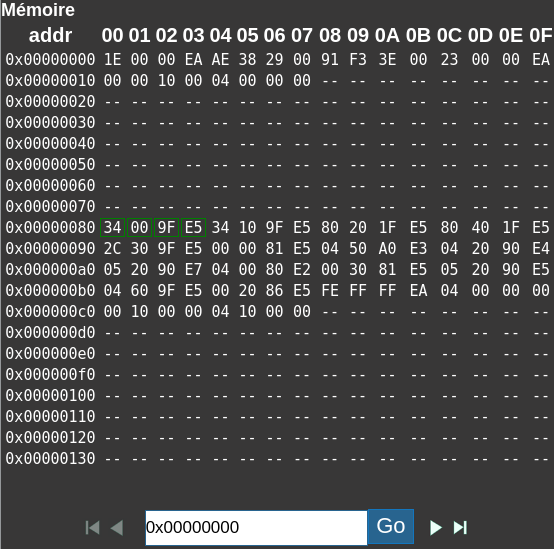
\includegraphics[width=0.9\linewidth]{pics/memoire.png}
\label{f:memoire}
\caption{Vue de la mémoire}
\end{marginfigure}
Tout comme pour les registres et les drapeaux, il est possible de modifier une valeur initialisée de la mémoire en cliquant. Les zones non déclarées (dont la valeur est identifiée par des tirets) ne peuvent être modifiées. La valeur doit être écrite en hexadécimal et ne peut excéder la capacité d'un octet (255, soit $0$xFF).

Lors de l'exécution, les octets composant l'instruction courante (celle surlignée en rouge dans l'éditeur) sont entourés de vert, comme dans l'exemple suivant :
\begin{figure}[h!]
\raggedleft
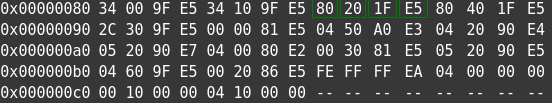
\includegraphics[width=0.8\linewidth]{pics/memoire_pc.png}
\label{f:memoirepc}
\caption{Affichage des octets composant l'instruction courante}
\end{figure}

Lorsque l'instruction est une opération agissant en mémoire, les cases mémoires lues ou écrites voient leurs valeurs colorées de manière différente (vert dans le cas d'une lecture, rouge dans le cas d'une écriture). Par exemple, dans l'image suivante, l'instruction courante lit les valeurs $0$x10 à $0$x13 inclusivement :
\begin{figure}[h!]
\raggedleft
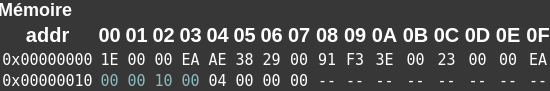
\includegraphics[width=0.8\linewidth]{pics/memoire_acces.png}
\label{f:memoireacces}
\caption{Exemple du changement de couleur des valeurs d'une case mémoire lors d'un accès}
\end{figure}

Il est possible de placer des points d'arrêt en mémoire. Ceux-ci peuvent être de trois types :
\begin{itemize}
	\item \textbf{Lecture} : le simulateur s'arrête lorsqu'un accès en lecture (par exemple via l'instruction LDR) est effectué sur cette case mémoire
	\item \textbf{Écriture} : le simulateur s'arrête lorsqu'un accès en écriture (par exemple via l'instruction STR) est effectué sur cette case mémoire
	\item \textbf{Exécution} : le simulateur s'arrête lorsque le \textit{Program Counter} (PC) atteint cette valeur
\end{itemize}
Notons que ces trois types de points d'arrêt peuvent être combinés. Par exemple, dans l'image suivante, un point d'arrêt en lecture est présent pour les adresses $0$x04 à $0$x07, un point d'arrêt en écriture est actif aux adresses $0$x0C à $0$x0F et un point d'arrêt en exécution est présent à l'adresse $0$x8C :
\begin{figure}[h!]
\raggedleft
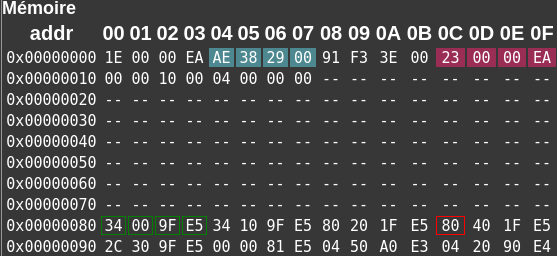
\includegraphics[width=0.8\linewidth]{pics/memoire_bkpt.png}
\label{f:memoirebkpt}
\caption{Exemple de points d'arrêt en mémoire. Un point d'arrêt en lecture peut être ajouté en cliquant sur une case mémoire tout en pressant la touche Control (Ctrl). Un point d'arrêt en écriture peut être ajouté en cliquant et pressant la touche Maj (Shift). Un point d'arrêt en écriture peut être ajouté en cliquant et pressant la touche Alt.}
\end{figure}

Afin de faciliter l'utilisation du simulateur, un aide-mémoire succinct reprenant les informations présentées ici est disponible en bas de la vue mémoire :
\begin{figure}[h!]
\raggedleft
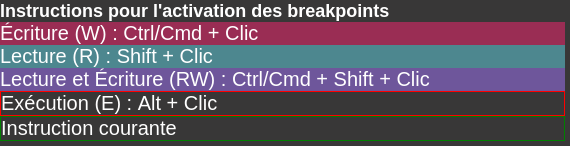
\includegraphics[width=0.8\linewidth]{pics/memoire_reminder.png}
\label{f:memoirerem}
\caption{Description des différents types de points d'arrêt en mémoire dans l'interface du simulateur}
\end{figure}

Finalement, en bas du visualisateur, on retrouve une interface permettant de naviguer dans la mémoire :
\begin{figure}[h!]
\raggedleft

\includegraphics[width=0.6\linewidth]{pics/memoire_goto.png}
\label{f:memoiregoto}
\caption{Contrôle de la position dans la mémoire}
\end{figure}

 Les flèches permettent d'aller vers des adresses mémoire plus hautes ou plus basses. Le champ de texte central permet de spécifier directement une adresse, à laquelle on peut par la suite se rendre en pressant le bouton \textit{Go}.

\clearpage

\subsection{Description de l'instruction courante}

Cette section présente des informations textuelles sur l'instruction courante. La première ligne présente l'instruction \emph{désassemblée} : elle provient non pas de l'éditeur, mais du \textit{bytecode} lui-même. Cela lui permet d'apporter de l'information supplémentaire dans deux circonstances :
\begin{enumerate}
	\item Les étiquettes y sont remplacées par les décalages effectifs requis pour atteindre la case mémoire demandée
	\item Dans le cas où l'on exécute des données présentes en mémoire, auxquelles aucun code assembleur n'est lié, cet affichage reste fonctionnel puisqu'il ne se base que sur la représentation binaire des instructions.
\end{enumerate}
\begin{figure}[h!]
\raggedleft
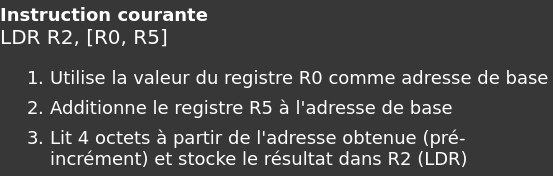
\includegraphics[width=0.6\linewidth]{pics/disassembly.png}
\label{f:disassembly}
\caption{Affichage de l'instruction désassemblée et de sa description. En fonction de l'instruction, la description peut être plus ou moins longue.}
\end{figure}

Les lignes suivantes sont une description textuelle de l'instruction, générée automatiquement. Elles indiquent, dans l'ordre, les opérations effectuées pour obtenir le résultat final et leurs effets de bord s'il y a lieu. Dans le cas d'une instruction indéfinie, cette zone reste vide.


\clearpage
\subsection{Contrôles d'enregistrement et de chargement}

Ces contrôles, situés au bas de l'écran, vous permettent de télécharger le code présent dans l'éditeur et de charger un code présent sur votre ordinateur. Ces deux actions sont analogues à l'ouverture et l'enregistrement dans une application traditionnelle.

\begin{figure}[h!]
\raggedleft

\includegraphics[width=0.9\linewidth]{pics/opensave.png}
\label{f:opensave}
\caption{Interface d'ouverture et d'enregistrement}
\end{figure}

N'importe quel type de fichier texte brut peut être lu par le simulateur. Nous vous recommandons toutefois d'utiliser l'extension ``txt'' afin d'éviter la confusion avec d'autres formats de fichier. C'est d'ailleurs cette extension que comportent les fichiers téléchargés depuis le simulateur.

\paragraph{\textbf{Note importante :}} ces contrôles constituent la \emph{seule} manière de sauvegarder et réouvrir votre code. Il n'y a \emph{aucun} système de sauvegarde automatique et le serveur ne conserve \emph{aucune} trace du code exécuté. \textbf{Si vous ne téléchargez pas votre code avant de fermer votre navigateur ou de changer de page, les modifications que vous y avez apportées seront perdues et irrécupérables.} Un message d'avertissement vous est présenté lorsque vous tentez de fermer la fenêtre afin de vous rappelez de télécharger le fichier.

\clearpage
\subsection{Configuration}

La fenêtre de configuration peut être ouverte en pressant le bouton \textit{Configurations} situé sous la vue des drapeaux. Une fois ouverte, la fenêtre ressemble à celle-ci :
\begin{figure}[h!]
\raggedleft
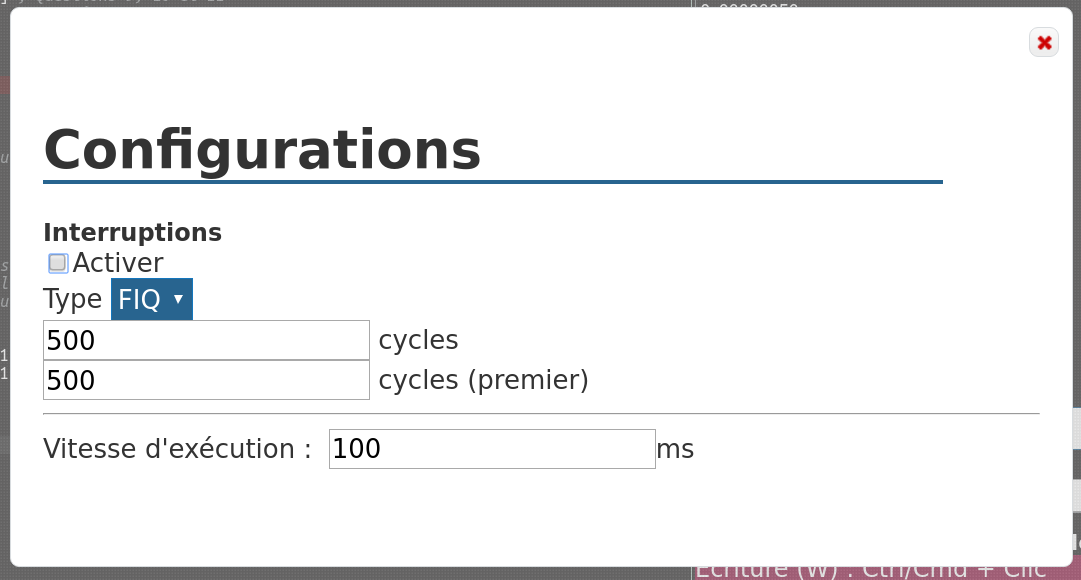
\includegraphics[width=0.9\linewidth]{pics/configurations.png}
\label{f:config}
\caption{Interface de configuration des interruptions et du simulateur}
\end{figure}

Deux éléments principaux peuvent être configurés dans cette interface :
\begin{enumerate}
	\item Une interruption temporelle peut être activée, en mode FIQ ou IRQ. Le nombre de cycles avant la première interruption, de même que le délai de répétition (encore là en nombre de cycles processeur) peuvent être configurés.
	\item La vitesse d'exécution, qui correspond au délai minimum entre l'exécution de deux instructions consécutives. Normalement, un délai de 100ms est suffisant pour exécuter les différents travaux pratiques et exercices du cours. Toutefois, dans certains cas spécifiques, une vitesse plus rapide peut être bénéfique. Dans tous les cas, n'oubliez pas que le simulateur ne peut exécuter plus qu'un certain nombre d'instructions à la suite, avant de se mettre en pause et d'attendre une nouvelle commande.
\end{enumerate}

\clearpage
\section{Instructions ARM supportées}

Le simulateur supporte les instructions suivantes. La syntaxe à utiliser est celle présentée dans les spécifications et documentations techniques d'ARM, sauf pour les spécificités suivantes :
\begin{enumerate}
	\item Toutes les mnémoniques (MOV, LDR, BL, etc.) doivent être écrites en \textbf{majuscules}
	\item Tous les noms de registres doivent être écrits en \textbf{majuscules}
	\item Les étiquettes peuvent être indifféremment en majuscules ou minuscules, mais ne peuvent être directement une mnémonique. Elles peuvent également contenir des chiffres, mais ne peuvent pas \textit{commencer} par un chiffre.
	\item L'indentation n'a pas d'importance. De même, l'espacement entre les différents composants d'une instruction n'est pas pris en compte, hormis pour l'espace ou la tabulation après la mnémonique, qui est obligatoire.
	\item Une \emph{section} se déclare uniquement par son nom. Les attributs de section (par exemple \textit{.noinit}) ne sont pas supportés.

\end{enumerate}

Référez-vous aux notes de cours ou à la documentation d'ARM pour plus de détails sur chacune de celles-ci.

\subsection{Suffixes conditionnels}
Toutes les instructions listées ci-dessous peuvent être exécutées \emph{conditionnellement}, en utilisant un des codes à 2 lettres suivants :
\begin{itemize}
	\item \textbf{EQ} teste l'égalité ($A == B$)
	\item \textbf{NE} teste l'inégalité ($A != B$)
	\item \textbf{CS} teste si un premier nombre non-signé est plus grand ou égal à un second ($A >= B$)
	\item \textbf{CC} teste si un premier nombre non-signé est strictement plus petit qu'un second ($A < B$)
	\item \textbf{MI} teste si le résultat est négatif ($A < 0$)
	\item \textbf{PL} teste si le résultat est positif ($A >= 0$)
	\item \textbf{VS} teste si la précédente opération a généré un \textit{débordement}
	\item \textbf{VC} teste si la précédente opération n'a PAS généré un \textit{débordement}
	\item \textbf{HI} teste si un premier nombre non-signé est plus grand à un second ($A > B$)
	\item \textbf{LS} teste si un premier nombre non-signé est plus petit ou égal à un second ($A <= B$)
	\item \textbf{GE} teste si un premier nombre est plus grand ou égal à un second ($A >= B$)
	\item \textbf{LT} teste si un premier nombre est strictement plus petit qu'un second ($A < B$)
	\item \textbf{GT} teste si un premier nombre est strictement plus grand qu'un second ($A > B$)
	\item \textbf{LE} teste si un premier nombre est plus petit ou égal à un second ($A > B$)
	\item \textbf{AL} exécute systématiquement l'instruction
\end{itemize}

\subsection{Instructions de manipulation de données}
\begin{itemize}
	\item MOV
	\item MVN
	\item ADD
	\item SUB
	\item MUL
	\item MLA
	\item AND
	\item EOR
	\item ORR
	\item ADC
	\item RSB
	\item SBC
	\item RSC
	\item BIC
	\item NOP
\end{itemize}

\subsection{Instructions de comparaison}
\begin{itemize}
	\item CMP
	\item CMN
	\item TST
	\item TEQ
\end{itemize}

\subsection{Instructions de décalage}
Note : ces instructions sont des pseudo-instructions. Elles sont transformées par le programme assembleur en une instruction MOV intégrant le décalage.
\begin{itemize}
	\item LSL
	\item LSR
	\item ASR
	\item ROR
	\item RRX
\end{itemize}

\subsection{Instructions de branchement}
\begin{itemize}
	\item B
	\item BL
	\item BX
\end{itemize}

\subsection{Instructions d'accès mémoire}
\begin{itemize}
	\item LDR
	\item STR
	\item LDRB
	\item STRB
\end{itemize}

\subsection{Instructions d'accès mémoire multiples}
\begin{itemize}
	\item LDM
	\item STM
	\item PUSH
	\item POP
\end{itemize}

\subsection{Instructions d'accès au registre de contrôle et de statut}
\begin{itemize}
	\item MSR
	\item MRS
\end{itemize}

\subsection{Instructions de déclenchement d'une interruption logicielle}
\begin{itemize}
	\item SWI
	\item SVC
\end{itemize}

\section{Remerciements}

Les auteurs tiennent à remercier les personnes suivantes pour l'aide qu'ils ont apporté à la réalisation de ce simulateur :
\begin{itemize}
	\item Jessica Déziel, pour le design de l'interface graphique
	\item Jonathan Gilbert, pour les tests préliminaires du simulateur et la réalisation des exercices
\end{itemize}

\end{document} 
